%!TEX root = ../docu.tex
\section{Konzept}

\subsection{Grundkonzept}

Das folgende Kapitel erläutert die Kozeptionierung der Anwendung, welche im späteren implementiert wird. Hierbei handelt es sich um eine Applikation hauptsächlich für das Abspielen von Hörbüchern im Audioformat MP3. Die Applikation ist so ausgelegt, das alle Funktionen einfach erreichbar und bedienbar sind.

Die Applikation soll dem Benutzer ermöglichen Hörbücher abzuspielen, welche er vorher auf sein mobiles Endgerät abgelegt hat. Hierfür muss die Applikation einen Einstellungsmöglichkeit beinhalten.

Über diese Einstellungen muss der Benutzer den Speicherort frei wählen und festlegen. Über diese Einstellungsparameter ist es der Anwendung nun möglich alle Audiodateien aufzulisten und abspielen zu können.

Die Auflistung filtert alle nicht abspielbaren Daten und ermöglicht des Weiteren in Unterordnen zu navigieren. Ein Element der Liste stellt dabei entweder eine Audiodatei oder ein Unterordner dar. 

\begin{figure}
\begin{center}
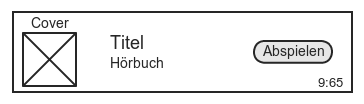
\includegraphics[scale=0.8]{images/listitem}
\caption{Mockup für ein Listenelement}
\label{mocklistel}
\end{center}
\end{figure}

Die Abbildung \ref{mocklistel} beschreibt ein solches Element. Ein Element enthält das Cover des Hörbuches sowie der Title und die genau Abspielzeit. Über ein weiteres Element ermöglicht eine Aktion, welche das Abspielen der jeweiligen Audiodatei auslöst.

Aus dieser Auflistung heraus werden alle Audiodateien abspielen die sich im jeweiligen aktuellen Verzeichnis befinden. Eine Schnittstelle zur Übertragung der Informationen zur Player Komponente realisiert diese Funktion.

Diese Komponente ist für das eigentliche Abspielen zuständig. Sie empfängt die Anweisung zum Abspielen der Audiodatei und spielt dieses Datei letztendlich ab.

\begin{figure}[ht]
\begin{minipage}[b]{0.45\linewidth}
\centering
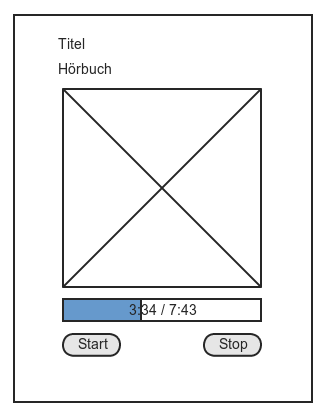
\includegraphics[width=\textwidth]{images/playerkomp}
\caption{Konzept des Players}
\label{playerkomp}
\end{minipage}
\hspace{0.5cm}
\begin{minipage}[b]{0.45\linewidth}
\centering
\fbox{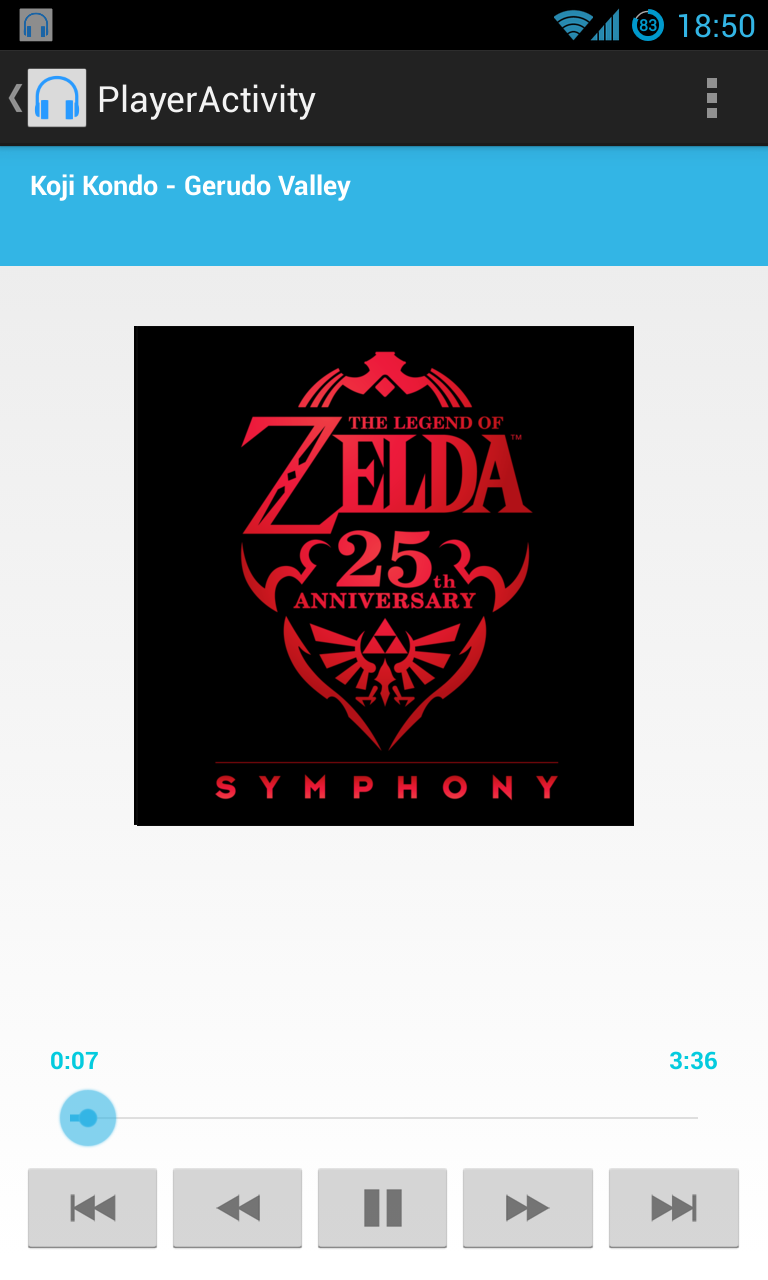
\includegraphics[width=\textwidth]{images/player_unframed}}
\caption{Player-Implementierung}
\label{player}
\end{minipage}
\end{figure}

Die Player Komponente in Abbildung \ref{playerkomp} dargestellt, ermöglicht es das Abspielen zu steuern. Dies beinhaltet das Stoppen, Pausieren und andere Funktionen. Des Weiteren ist Erkennbarkeit welche Audiodatei abgespielt wird. Eine Vorschrittanzeige lässt erkennen, wie viel von der Audiodatei bisher abgespielt wird sowie die Gesamtlänge der Audiodatei.

\begin{figure}
\begin{center}
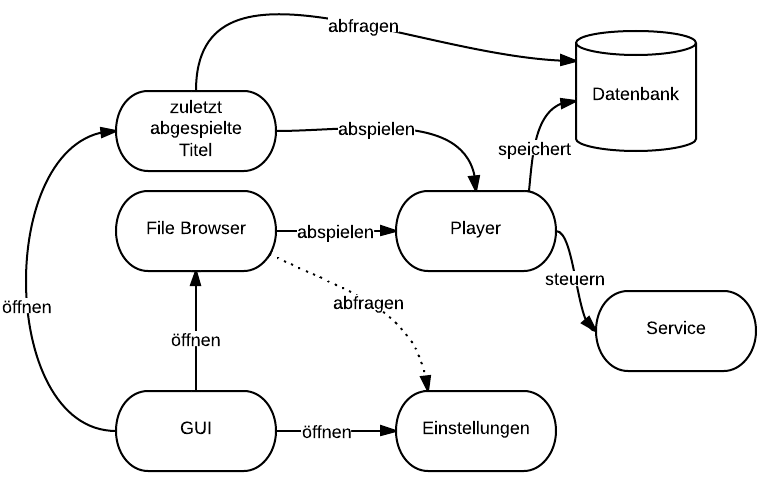
\includegraphics[scale=0.6]{images/konzept}
\caption{Schematische Darstellung der Anwendung}
\label{konzept}
\end{center}
\end{figure}

Wird die Anwendung geschlossen wird die Wiedergebe abgebrochen. Sie ist in der Lage Abbrüche der Wiedergabe zu erkennen und diese Punkte zu Speicher. Der Benutzer hat eine Möglichkeit, die Wiedergabe an diesen Punkten de Wiedergabe vorzusetzen.

Die Eingabe erfolgt durch ein übliches Touchscreen Display und ist dahingehen optimiert. Hierzu gehört klare und einfache Programmstrukturen sowie ausreichend große Fälschen für Bedienelemente und Steuerung von Programmfunktionen.

Die gesamte Programmstruktur ist so aufgebaut, dass eine Weiterentwicklung und Implementierung neuer Funktionen möglich ist.